\subsection*{3.4 Two Variable Data: Models and Scatterplots}
\vspace{0.5em}

\setcounter{questionnum}{0}

\noindent\markforreview
\vspace{1em}

\begin{center}
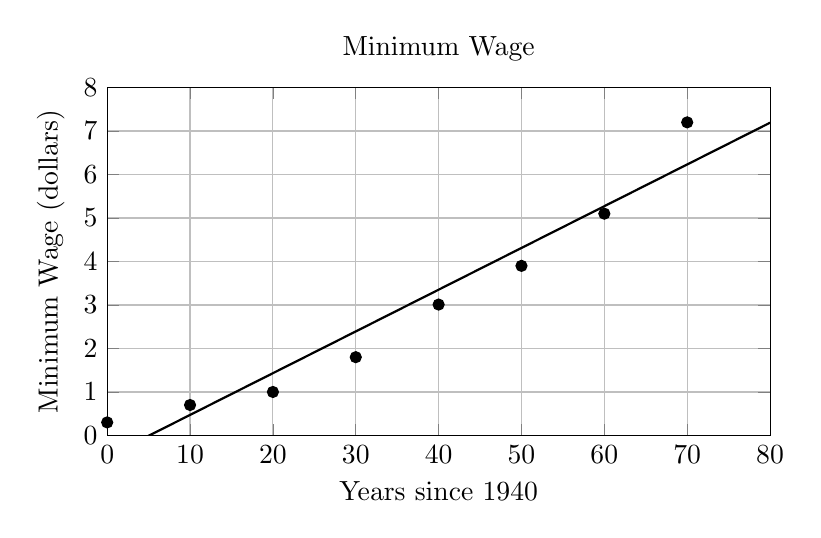
\begin{tikzpicture}
\begin{axis}[
    xlabel={Years since 1940},
    ylabel={Minimum Wage (dollars)},
    ytick={0,1,...,8},
    xmin=0, xmax=80,
    ymin=0, ymax=8,
    grid=major,
    width=10cm, height=6cm,
    title={Minimum Wage}
]
\addplot[
    only marks,
    mark=*,
    samples at={0,10,20,30,40,50,60,70},
]
coordinates {
    (0, 0.3)
    (10, 0.7)
    (20, 1)
    (30, 1.8)
    (40, 3.01)
    (50, 3.9)
    (60, 5.1)
    (70, 7.2)
};
\addplot[domain=0:80, thick] {0.096*x - 0.488};
\end{axis}
\end{tikzpicture}

\end{center}

The scatterplot above shows the federal-mandated minimum wage every 10 years between 1940 and 2010.  
A line of best fit is shown, and its equation is $y = 0.096x - 0.488$.  
What does the line of best fit predict about the increase in the minimum wage over the 70-year period?

\vspace{0.75em}

\choicebox{A}{Each year between 1940 and 2010, the average increase in minimum wage was 0.096 dollars.}  
\choicebox{B}{Each year between 1940 and 2010, the average increase in minimum wage was 0.49 dollars.}  
\choicebox{C}{Every 10 years between 1940 and 2010, the average increase in minimum wage was 0.096 dollars.}  
\choicebox{D}{Every 10 years between 1940 and 2010, the average increase in minimum wage was 0.488 dollars.}

\newpage

\noindent\markforreview
\vspace{1em}

\begin{center}
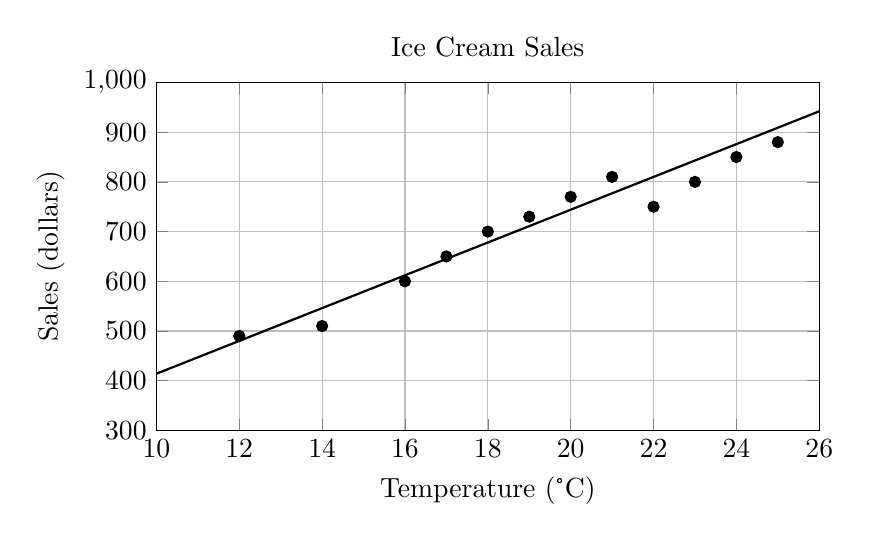
\begin{tikzpicture}
\begin{axis}[
    xlabel={Temperature (°C)},
    ylabel={Sales (dollars)},
    ytick={300,400,...,1000},
    xmin=10, xmax=26,
    ymin=300, ymax=1000,
    grid=major,
    width=10cm, height=6cm,
    title={Ice Cream Sales}
]
\addplot[
    only marks,
    mark=*,
]
coordinates {
    (12, 490)
    (14, 510)
    (16, 600)
    (17, 650)
    (18, 700)
    (19, 730)
    (20, 770)
    (21, 810)
    (22, 750)
    (23, 800)
    (24, 850)
    (25, 880)
};
\addplot[domain=10:26, thick] {33*x + 84};
\end{axis}
\end{tikzpicture}

\end{center}

The scatterplot above shows a company’s ice cream sales $d$, in dollars, and the high temperature $t$, in degrees Celsius (°C), on 12 different days.  
A line of best fit for the data is also shown.  
Which of the following could be an equation of the line of best fit?

\vspace{0.75em}

\choicebox{A}{$d = 0.03t + 402$}  
\choicebox{B}{$d = 10t + 402$}  
\choicebox{C}{$d = 33t + 300$}  
\choicebox{D}{$d = 33t + 84$}

\newpage


\noindent\markforreview
\vspace{1em}
\begin{center}
    

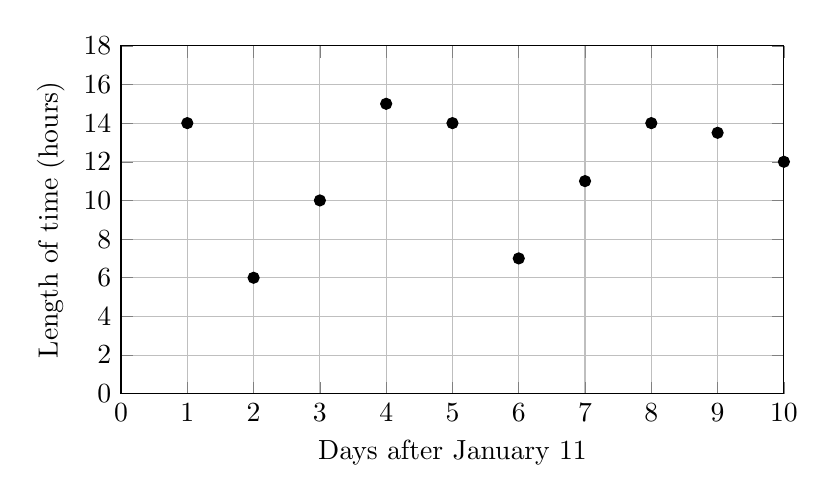
\begin{tikzpicture}
\begin{axis}[
    xlabel={Days after January 11},
    ylabel={Length of time (hours)},
    xmin=0, xmax=10,
    ymin=0, ymax=18,
    grid=major,
    width=10cm, height=6cm,
    ytick={0,2,...,18},
    xtick={0,1,...,10}
]
\addplot[
    only marks,
    mark=*,
    black
] coordinates {
    (1,14) (2,6) (3,10) (4,15) (5,14)
    (6,7) (7,11) (8,14) (9,13.5) (10,12)
};
\end{axis}
\end{tikzpicture}
\end{center}


The scatterplot shows the relationship between the length of time $y$, in hours, a certain bird spent in flight and the number of days after January 11, $x$.

What is the average rate of change, in hours per day, of the length of time the bird spent in flight on January 13 to the length of time the bird spent in flight on January 15?

\vspace{2em}

\noindent\markforreview
\vspace{1em}

\begin{center}
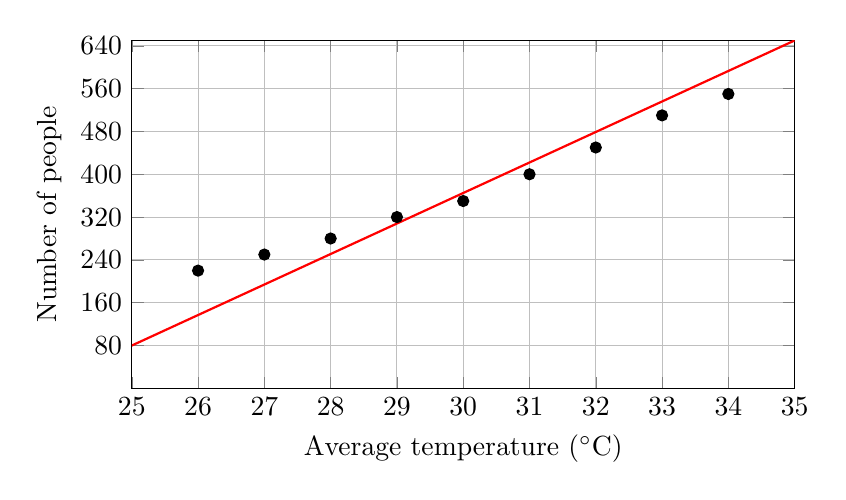
\begin{tikzpicture}
\begin{axis}[
    xlabel={Average temperature ($^\circ$C)},
    ylabel={Number of people},
    xtick={25,26,...,35},
    ytick={80,160,...,640},
    xmin=25, xmax=35,
    ymin=0, ymax=650,
    grid=major,
    width=10cm, height=6cm
]
\addplot[only marks, mark=*] coordinates {
    (26,220) (27,250) (28,280) (29,320) (30,350)
    (31,400) (32,450) (33,510) (34,550)
};
\addplot[red, thick, domain=25:35, samples=2] {57*x - 1345};
\end{axis}
\end{tikzpicture}

\end{center}



Each dot in the scatterplot above represents the temperature and the number of people who visited a beach in Lagos, Nigeria, on one of eleven different days.  
The line of best fit for the data is also shown.  
The line of best fit has a slope of approximately $57$.  
According to this estimate, how many additional people per day are predicted to visit the beach for each $5^\circ$C increase in average temperature?

\newpage

\noindent\markforreview
\vspace{1em}

\begin{center}
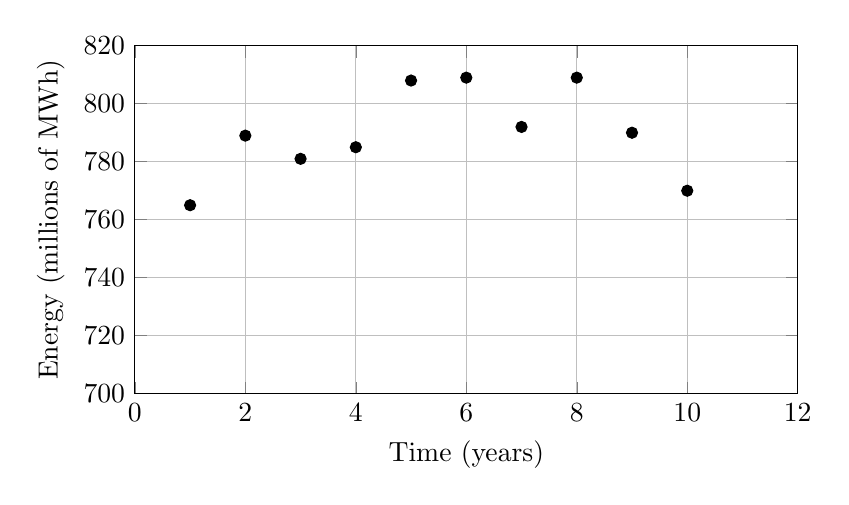
\begin{tikzpicture}
\begin{axis}[
    xlabel={Time (years)},
    ylabel={Energy (millions of MWh)},
    xtick={0,2,...,12},
    ytick={700,720,...,820},
    xmin=0, xmax=12,
    ymin=700, ymax=820,
    grid=major,
    width=10cm, height=6cm
]
\addplot[only marks, mark=*] coordinates {
     (1,765) (2,789) (3,781) (4,785)
    (5,808) (6,809) (7,792) (8,809) (9,790) (10,770)
};
\addplot[blue, thick, domain=0:10] {1.674*x^2 + 19.76*x - 745.73};
\end{axis}
\end{tikzpicture}

\end{center}

The scatterplot below shows the amount of electric energy generated, in millions of megawatt-hours, by nuclear sources over a 10-year period.

Of the following equations, which best models the data in the scatterplot?

\vspace{0.75em}

\choicebox{A}{$y = 1.674x^2 + 19.76x - 745.73$}
\choicebox{B}{$y = -1.674x^2 - 19.76x - 745.73$}
\choicebox{C}{$y = 1.674x^2 + 19.76x + 745.73$}
\choicebox{D}{$y = -1.674x^2 + 19.76x + 745.73$}

\vspace{2em}


\newpage
\noindent\markforreview
\vspace{1em}

\begin{center}
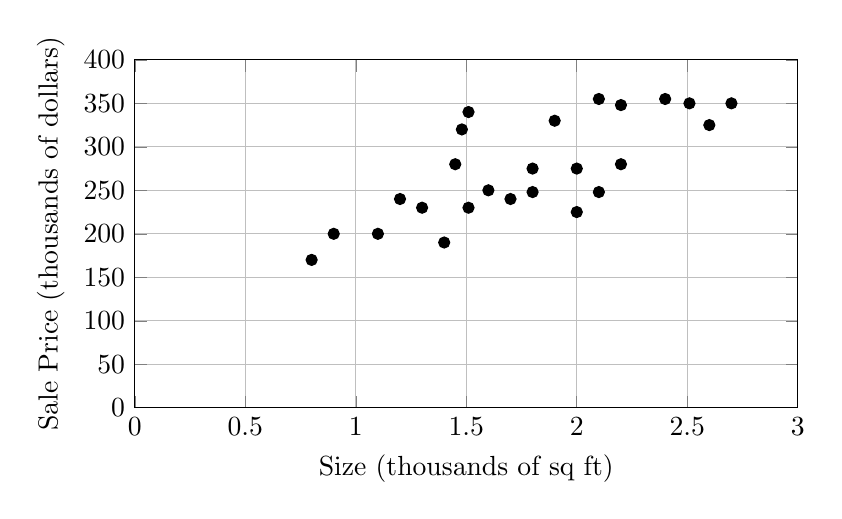
\begin{tikzpicture}
\begin{axis}[
    xlabel={Size (thousands of sq ft)},
    ylabel={Sale Price (thousands of dollars)},
        xtick={0,0.5,...,3},
    ytick={0,50,...,400},
    xmin=0, xmax=3.0,
    ymin=0, ymax=400,
    grid=major,
    width=10cm, height=6cm
]
\addplot[only marks, mark=*] coordinates {
    (0.8,170) (0.9,200) (1.1,200) (1.2,240) (1.3,230)(1.4,190)(1.45,280)(1.48,320)(1.51,340)(1.51,230)(1.6,250)(1.7,240)(1.8,248)(1.8,275)(1.9,330)(2,225)(2.0,275)(2.1,248)(2.1,355)(2.2,280)(2.2,348)(2.4,355)
    (2.51,350) (2.6,325) (2.7,350) 
};

\end{axis}
\end{tikzpicture}

\end{center}

The scatterplot above shows the size $x$ and the sale price $y$ of 25 houses for sale in Town H.  
Which of the following could be an equation for a line of best fit for the data?

\vspace{0.75em}

\choicebox{A}{$y = 200x + 100$}
\choicebox{B}{$y = 100x + 100$}
\choicebox{C}{$y = 50x + 100$}
\choicebox{D}{$y = 100x$}

\newpage

\noindent\markforreview
\vspace{1em}

For $x > 0$, the function $f$ is defined as follows:  
\begin{center}

$f(x)$ equals $201\%$ of $x$.
\end{center}

Which of the following could describe this function?

\vspace{0.75em}

\choicebox{A}{Decreasing exponential}
\choicebox{B}{Decreasing linear}
\choicebox{C}{Increasing exponential}
\choicebox{D}{Increasing linear}


\vspace{2em}
\noindent\markforreview
\vspace{1em}

\begin{center}
\begin{tabular}{|c|c|c|}
\hline
& \textbf{Amount invested} & \textbf{Balance increase} \\
\hline
\textbf{Account A} & \$500 & 6\% annual interest \\
\textbf{Account B} & \$1,000 & \$25 per year \\
\hline
\end{tabular}
\end{center}

Two investments were made as shown in the table above.  
The interest in Account A is compounded once per year.  
Which of the following is true about the investments?

\vspace{0.75em}

\choicebox{A}{Account A always earns more money per year than Account B.}
\choicebox{B}{Account A always earns less money per year than Account B.}
\choicebox{C}{Account A earns more money per year than Account B at first but eventually earns less money per year.}
\choicebox{D}{Account A earns less money per year than Account B at first but eventually earns more money per year.}

\vspace{2em}
\newpage
\noindent\markforreview
\vspace{1em}

\begin{center}
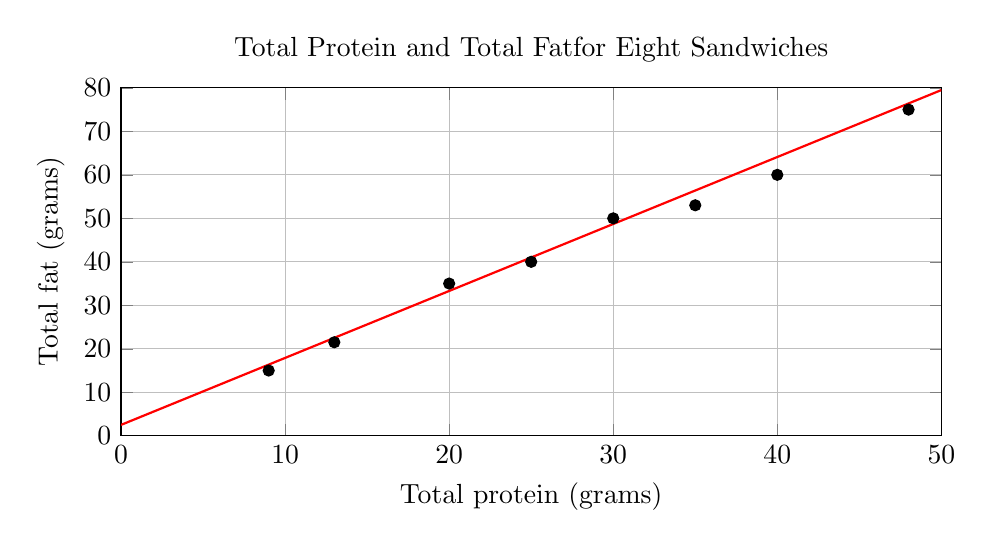
\begin{tikzpicture}
\begin{axis}[
    xlabel={Total protein (grams)},
    ylabel={Total fat (grams)},
    title={Total Protein and Total Fat\\for Eight Sandwiches},
    xmin=0, xmax=50,
    ymin=0, ymax=80,
    xtick={0,10,20,30,40,50},
    ytick={0,10,20,30,40,50,60,70,80},
    grid=major,
    width=12cm, height=6cm,
    legend style={at={(0.98,0.05)}, anchor=south east}
]

% Scatterplot points (estimated visually)
\addplot[only marks, mark=*] coordinates {
    (9, 15) (13, 21.5) (20, 35) (25, 40)
    (30, 50) (35, 53) (40, 60) (48,75 )
};

% Best fit line (from previous slope estimation: y = 1.29x + 2.39)
\addplot[red, thick, domain=0:50] {1.54*x + 2.5};


\end{axis}
\end{tikzpicture}

\end{center}

The scatterplot above shows the numbers of grams of both total protein and total fat for eight sandwiches on a restaurant menu.  
The line of best fit for the data is also shown.  
According to the line of best fit, which of the following is closest to the predicted increase in total fat, in grams,  
for every increase of 1 gram in total protein?

\vspace{0.75em}

\choicebox{A}{$2.5$}
\choicebox{B}{$2.0$}
\choicebox{C}{$1.5$}
\choicebox{D}{$1.0$}


\newpage
